
\subsection{Two-dimensional Poisson Equation}

\begin{figure}[!h]
  \centering
  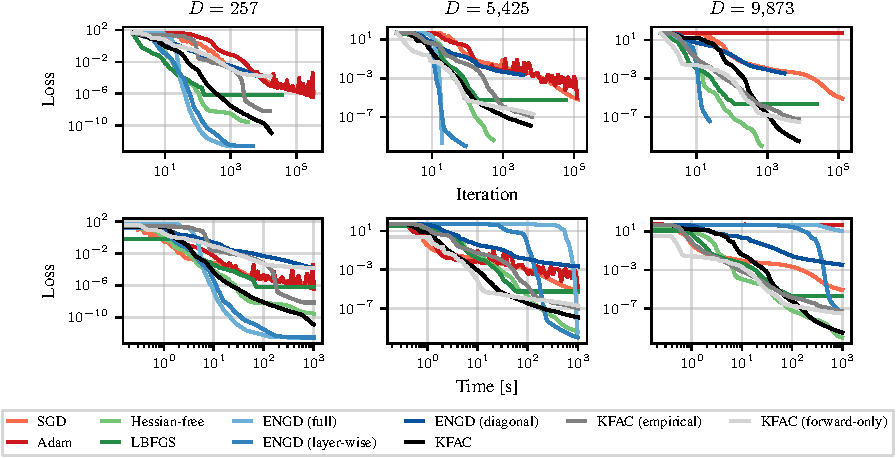
\includegraphics{../kfac_pinns_exp/exp17_groupplot_poisson2d/loss_all.pdf}
  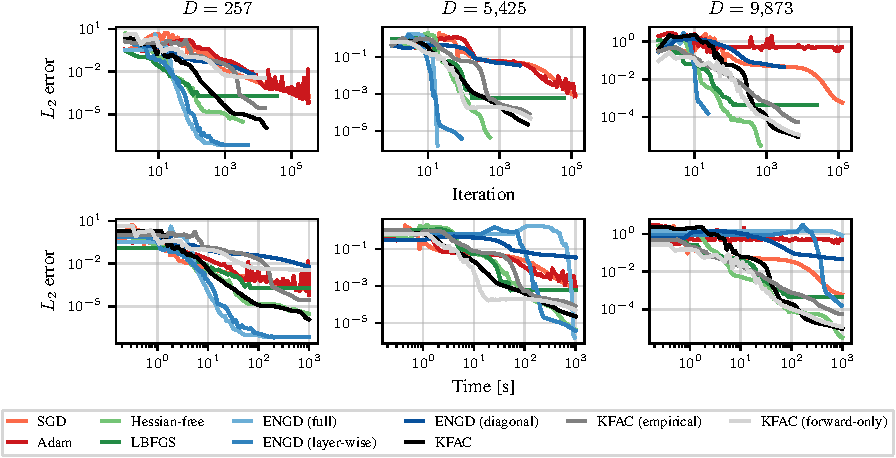
\includegraphics{../kfac_pinns_exp/exp17_groupplot_poisson2d/l2_error_all.pdf}
  \caption{$L_2$-error for learning the solution of a 2d-Poisson equation with different neural network size under a given time budget of $10^3\,\text{s}$ on an RTX 6000 GPU.}
\end{figure}

\clearpage

\subsection{Five-dimensional Poisson Equation}

\begin{figure}[!h]
  \centering
  \begin{subfigure}{0.325\linewidth}
    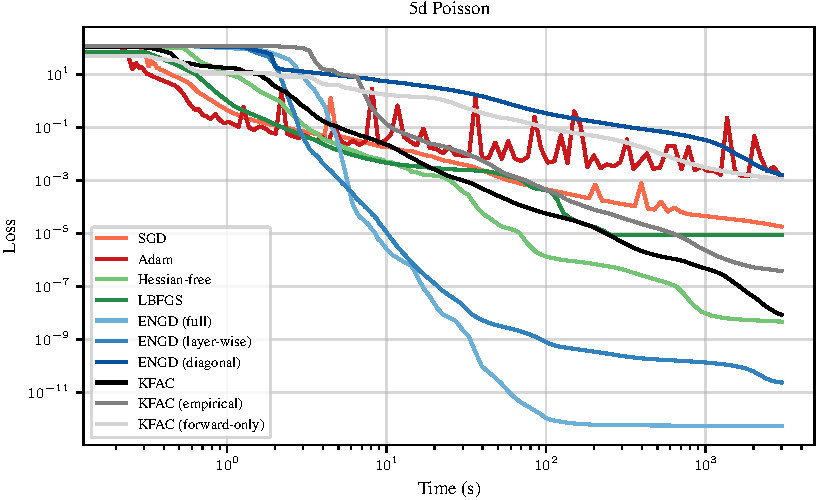
\includegraphics[width=\linewidth]{../kfac_pinns_exp/exp10_reproduce_poisson5d/loss_over_time}
    \\
    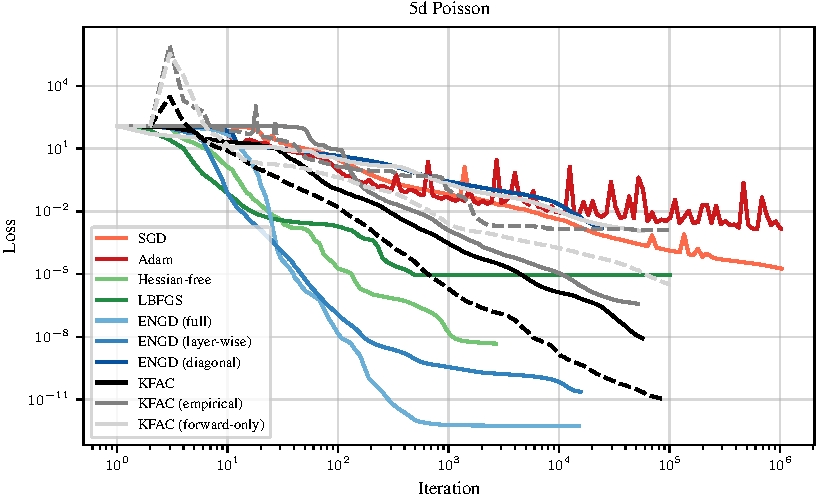
\includegraphics[width=\linewidth]{../kfac_pinns_exp/exp10_reproduce_poisson5d/loss_over_step}
    \caption{$\dim(\Omega) = 5, D = 449$}
  \end{subfigure}
  \hfill
  \begin{subfigure}{0.325\linewidth}
    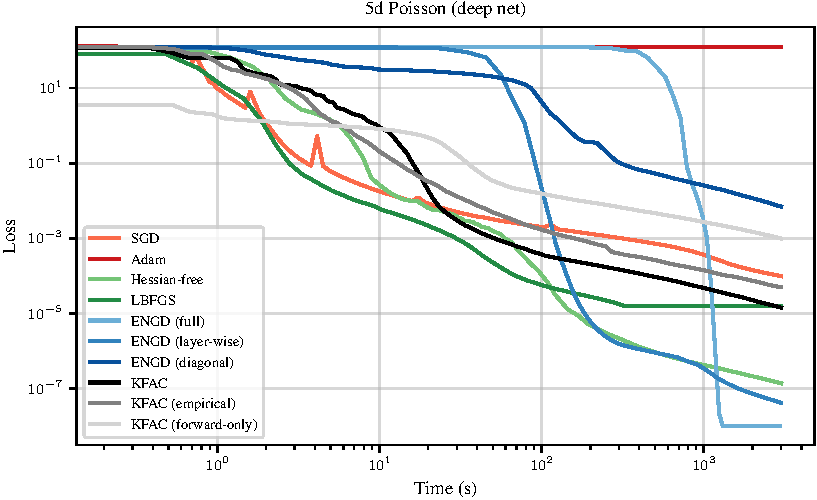
\includegraphics[width=\linewidth]{../kfac_pinns_exp/exp12_poisson5d_deep/loss_over_time}
    \\
    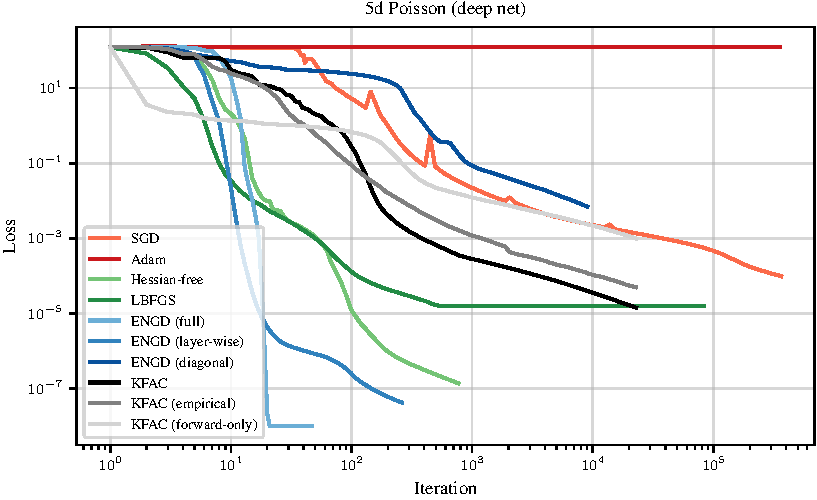
\includegraphics[width=\linewidth]{../kfac_pinns_exp/exp12_poisson5d_deep/loss_over_step}
    \caption{$\dim(\Omega) = 5, D = 5,617$}
  \end{subfigure}
  \hfill
  \begin{subfigure}{0.325\linewidth}
    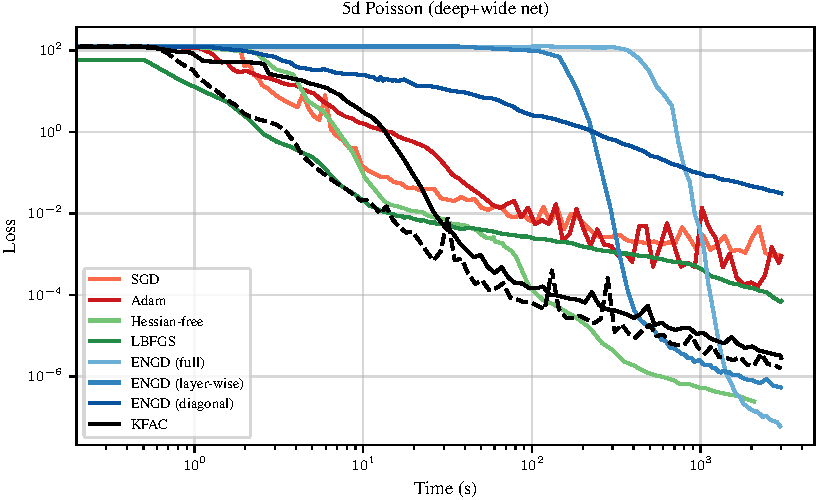
\includegraphics[width=\linewidth]{../kfac_pinns_exp/exp16_poisson5d_deepwide/loss_over_time}
    \\
    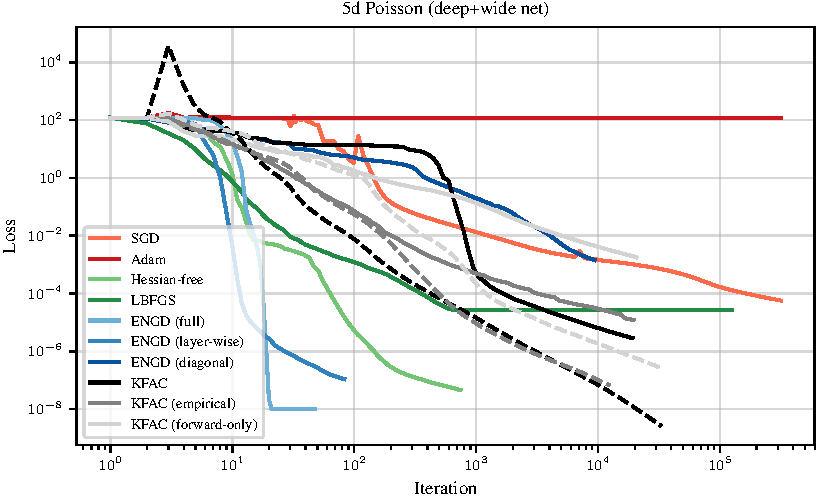
\includegraphics[width=\linewidth]{../kfac_pinns_exp/exp16_poisson5d_deepwide/loss_over_step}
    \caption{$\dim(\Omega) = 5, D = 10,065$}
  \end{subfigure}
  \caption{Loss curves for learning the solution of a 5d-Poisson equation with different neural network size under a given time budget of $3\cdot 10^3\,\text{s}$ on an RTX 6000 GPU.
    Top row shows loss over time, bottom row shows loss over step.
    \felix{Discuss which optimizers to show.
      Create a pretty version using a 2x3 subplot.
    }}
\end{figure}

\begin{figure}[!h]
  \centering
  \begin{subfigure}{0.325\linewidth}
    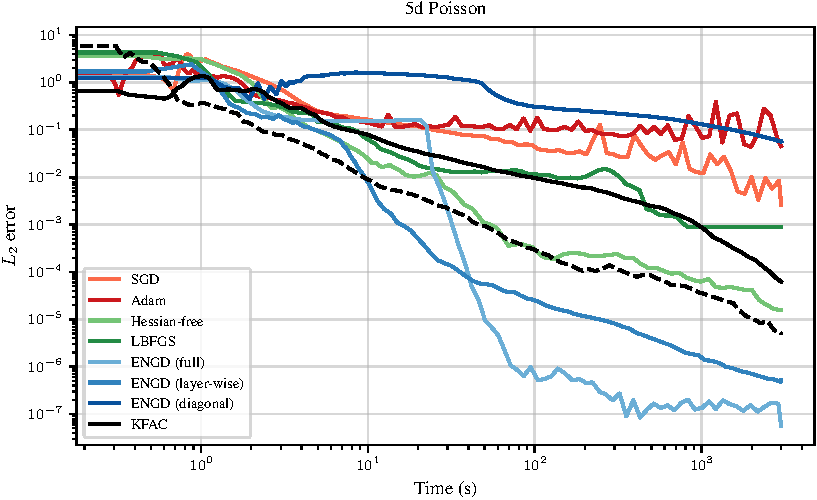
\includegraphics[width=\linewidth]{../kfac_pinns_exp/exp10_reproduce_poisson5d/l2_error_over_time}
    \\
    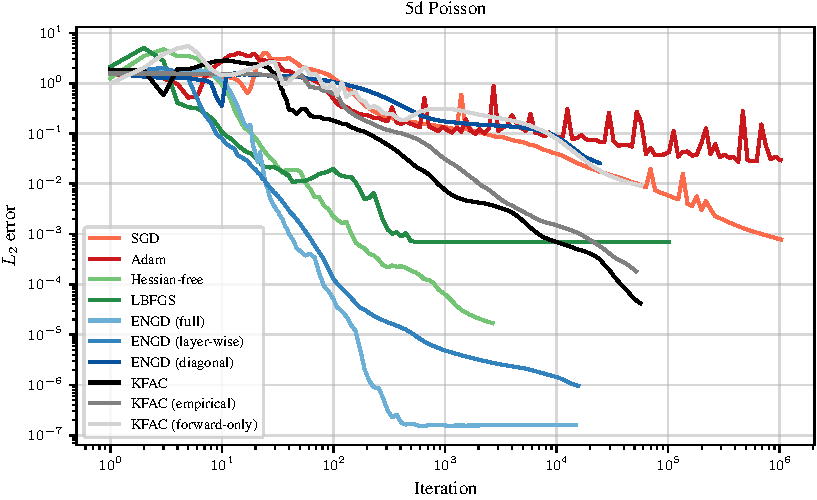
\includegraphics[width=\linewidth]{../kfac_pinns_exp/exp10_reproduce_poisson5d/l2_error_over_step}
    \caption{$\dim(\Omega) = 5, D = 449$}
  \end{subfigure}
  \hfill
  \begin{subfigure}{0.325\linewidth}
    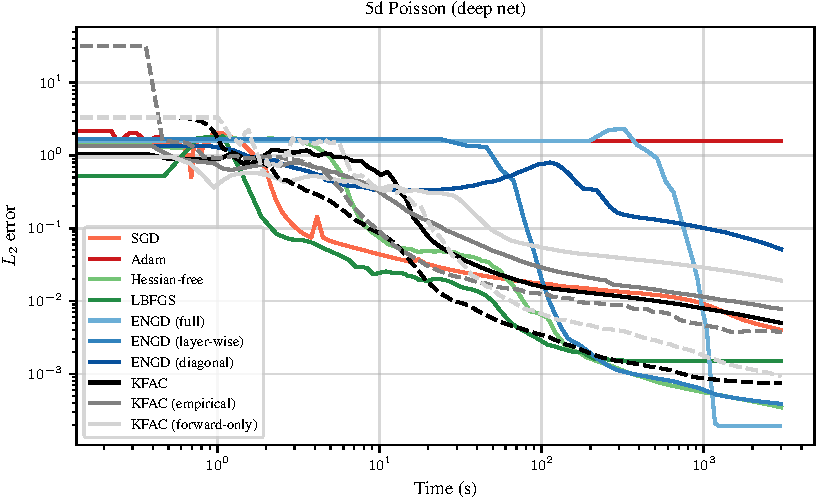
\includegraphics[width=\linewidth]{../kfac_pinns_exp/exp12_poisson5d_deep/l2_error_over_time}
    \\
    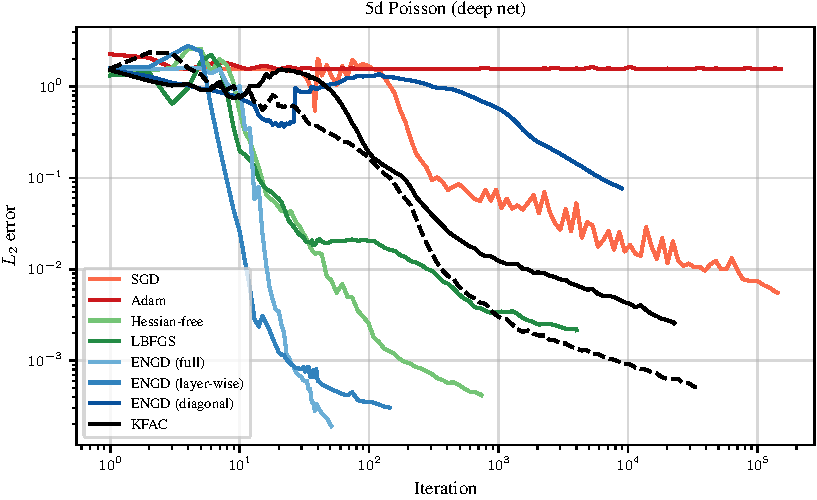
\includegraphics[width=\linewidth]{../kfac_pinns_exp/exp12_poisson5d_deep/l2_error_over_step}
    \caption{$\dim(\Omega) = 5, D = 5,617$}
  \end{subfigure}
  \hfill
  \begin{subfigure}{0.325\linewidth}
    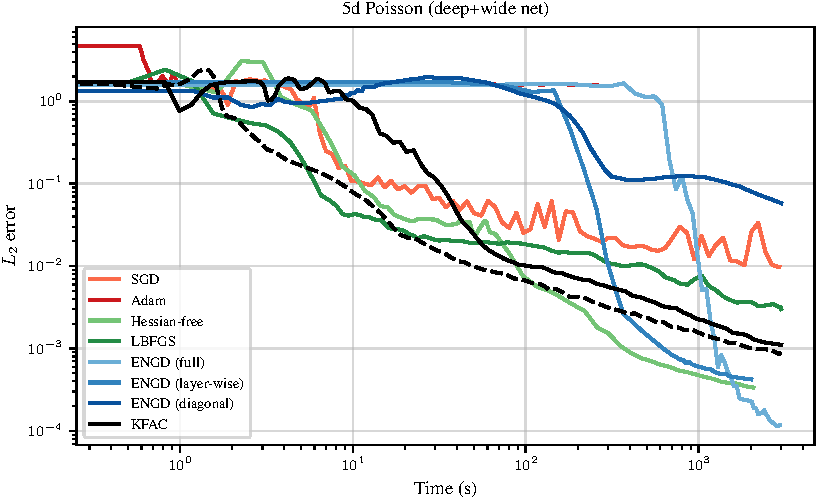
\includegraphics[width=\linewidth]{../kfac_pinns_exp/exp16_poisson5d_deepwide/l2_error_over_time}
    \\
    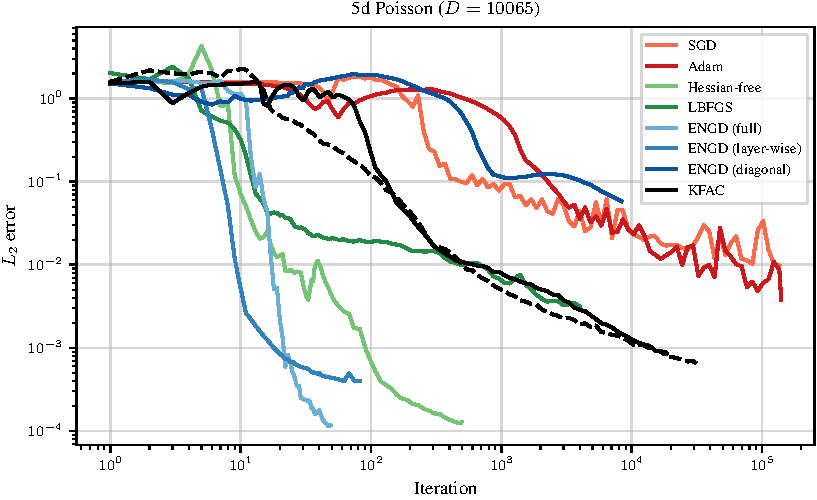
\includegraphics[width=\linewidth]{../kfac_pinns_exp/exp16_poisson5d_deepwide/l2_error_over_step}
    \caption{$\dim(\Omega) = 5, D = 10,065$}
  \end{subfigure}
  \caption{$L_2$-error for learning the solution of a 5d-Poisson equation with different neural network size under a given time budget of $3\cdot 10^3\,\text{s}$ on an RTX 6000 GPU.
    Top row shows $L_2$ error over time, bottom row shows $L_2$ error over step.
    \felix{Discuss which optimizers to show.
      Create a pretty version using a 2x3 subplot.
    }}
\end{figure}

%%% Local Variables:
%%% mode: latex
%%% TeX-master: "../main"
%%% End:
